\themaN
\graphicspath{{../../S26_Somme_et_difference_de_fractions/Images/}}

\chapter{Somme et différence\\de fractions}
\label{S26}



%%%%%%%%%%%%%%%%%%%%%%%%%%%%%%%%%%%%%%%%%%
\begin{prerequis}
   \begin{itemize}
      \item Somme, différence de deux nombres rationnels.
      \item[\com] Calculer avec des fractions.
      \item[\com] Effectuer des calculs et des comparaisons pour traiter des problèmes.
   \end{itemize}
\end{prerequis}

\vfill

\begin{debat}[Débat : l'\oe il d'Oudjat, ou \oe il d'Horus] 
   Dans la mythologie égyptienne, on trouve une histoire liée aux fractions : {\it Seth}, dieu de la violence et incarnation du mal, arrache l’{\bf œil} à {\bf Horus}. {\it Seth} le partage en six morceaux et les répand à travers l’Egypte. {\it Thot}, dieu magicien, reconstitue l’œil, symbole du bien contre le mal. Chacune de ses parties symbolise une fraction de numérateur 1 et de dénominateurs 2, 4, 8, 16, 32 et 64. Il accordera le 64\up{e} manquant à tout scribe recherchant et acceptant sa protection.
   \begin{center}
      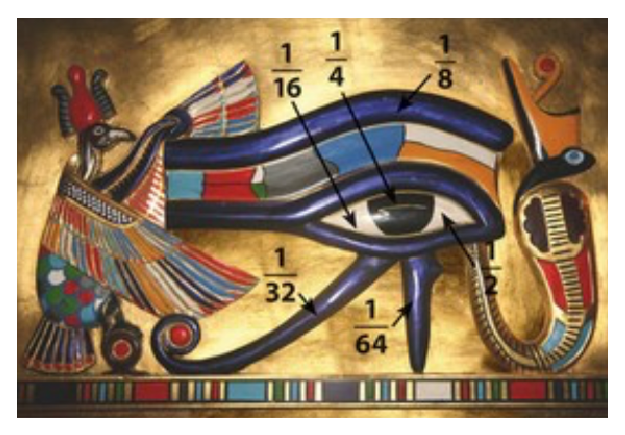
\includegraphics[width=6cm]{Horus}
   \end{center}
   \bigskip
   \begin{cadre}[B2][F4]
      \begin{center}
         Vidéo : \href{https://www.youtube.com/watch?v=yHft4m1Gi7k}{\bf La légende de l'\oe il d'Horus}, chaîne YouTube {\it Ma deuxième école}, épisode de la série {\it Culture G}.
      \end{center}
   \end{cadre}
\end{debat}

\vfill

\textcolor{PartieGeometrie}{\sffamily\bfseries Cahier de compétences} : chapitre 2, exercices 30 à 41 ; 46 à 49.


%%%%%%%%%%%%%%%%%%%%%%%%%%%%%%%%%%%%%%
%%%%%%%%%%%%%%%%%%%%%%%%%%%%%%%%%%%%%%
\activites

\begin{activite}[Décomposer une fraction]
   {\bf Objectifs :} représenter des fractions ; écrire une fraction sous la forme de la somme ou de la différence d'un entier et d'une fraction inférieure à 1.
   \begin{QCM}
      \partie[des toasts en entrée]
         Pour faire des toasts à ses amis, Chiara coupe des tranches de pain de mie en quatre, avant de les garnir. \\
         Maryam mange onze de ces petits toasts. Quelle fraction de grande tranche de pain de mie Mariam a-t-elle mangée ?
         \begin{center}
            {\psset{unit=0.9}
            \begin{pspicture}(0,0)(3,1.5)
               \psframe[fillstyle=solid,fillcolor=G2](0,0)(2,1.5)
               \psline(1,0)(1,1.5)
               \psline(0,0.75)(2,0.75)
            \end{pspicture}
            \begin{pspicture}[fillstyle=solid,fillcolor=G2](0,0)(3,1.5)
               \psframe(0,0)(2,1.5)
               \psline(1,0)(1,1.5)
               \psline(0,0.75)(2,0.75)
            \end{pspicture}
            \begin{pspicture}(0,0)(3,1.5)
               \psframe(0,0)(2,1.5)
               \pspolygon[fillstyle=solid,fillcolor=G2](0,0)(1,0)(1,0.75)(2,0.75)(2,1.5)(0,1.5)
               \psline(1,0)(1,1.5)
               \psline(0,0.75)(2,0.75)
            \end{pspicture}
            \begin{pspicture}(0,0)(3,1.5)
               \psframe(0,0)(2,1.5)
               \psline(1,0)(1,1.5)
               \psline(0,0.75)(2,0.75)
            \end{pspicture}
            \begin{pspicture}(0,0)(3,1.5)
               \psframe(0,0)(2,1.5)
               \psline(1,0)(1,1.5)
               \psline(0,0.75)(2,0.75)
            \end{pspicture}}
         \end{center}
         Elle a mangé 11 fois $\dfrac14$ de grande tranche, donc $\dfrac{11}4$ de grande tranche, ce qui fait 2 tranches et $\dfrac34$ de tranche, ou \\ [1mm]
3 tranches moins $\dfrac14$ de tranche. On peut écrire : $\dfrac{11}4 =2+\dfrac34 =3-\dfrac14$. \\ [1mm]
         Maïssa, elle, a mangé 17 petits toasts. Colorier ce que cela représente ci-dessous.
         \begin{center}
            {\psset{unit=0.9}
            \begin{pspicture}(0,0)(3,1.5)
               \psframe(0,0)(2,1.5)
               \psline(1,0)(1,1.5)
               \psline(0,0.75)(2,0.75)
            \end{pspicture}
            \begin{pspicture}(0,0)(3,1.5)
               \psframe(0,0)(2,1.5)
               \psline(1,0)(1,1.5)
               \psline(0,0.75)(2,0.75)
            \end{pspicture}
            \begin{pspicture}(0,0)(3,1.5)
               \psframe(0,0)(2,1.5)
               \pspolygon(0,0)(1,0)(1,0.75)(2,0.75)(2,1.5)(0,1.5)
               \psline(1,0)(1,1.5)
               \psline(0,0.75)(2,0.75)
            \end{pspicture}
            \begin{pspicture}(0,0)(3,1.5)
               \psframe(0,0)(2,1.5)
               \psline(1,0)(1,1.5)
               \psline(0,0.75)(2,0.75)
            \end{pspicture}
            \begin{pspicture}(0,0)(3,1.5)
               \psframe(0,0)(2,1.5)
               \psline(1,0)(1,1.5)
               \psline(0,0.75)(2,0.75)
            \end{pspicture}}
         \end{center}
         Compléter l'égalité  : \hspace{30mm} $\dfrac{17}4 = {\hdashrule{1cm}{0.15pt}{4pt 2pt}} + \dfrac{\hdashrule{1cm}{0.15pt}{4pt 2pt}}{\hdashrule{1cm}{0.15pt}{4pt 2pt}} ={\hdashrule{1cm}{0.15pt}{4pt 2pt}} - \dfrac{\hdashrule{1cm}{0.15pt}{4pt 2pt}}{\hdashrule{1cm}{0.15pt}{4pt 2pt}}$ \\

      \partie[des \og flam \fg{} en plat principal]
         Pour poursuivre, Chiara propose à ses amis de manger des flammekueches (flam). \\
         \begin{minipage}{7.75cm}
            \begin{pspicture}(-1.2,-1)(1,1)
               \pscircle[fillstyle=solid,fillcolor=G2](0,0){0.7}
               \multido{\n=0+72}{5}{\psline(0,0)(0.7;\n)}
            \end{pspicture}
            \begin{pspicture}(-0.7,-1)(1,1)
               \pscircle(0,0){0.7}
               \pswedge[fillstyle=solid,fillcolor=G2](0,0){0.7}{72}{288}
               \multido{\n=0+72}{5}{\psline(0,0)(0.7;\n)}
            \end{pspicture}
            \begin{pspicture}(-0.7,-1)(1,1)
               \pscircle(0,0){0.7}
               \multido{\n=0+72}{5}{\psline(0,0)(0.7;\n)}
            \end{pspicture}
            \begin{pspicture}(-0.7,-1)(1,1)
               \pscircle(0,0){0.7}
               \multido{\n=0+72}{5}{\psline(0,0)(0.7;\n)}
            \end{pspicture} \\
            Une part de flam représente $\dfrac{\hdashrule{1cm}{0.15pt}{4pt 2pt}}{\hdashrule{1cm}{0.15pt}{4pt 2pt}}$ de flam. \\ [3mm]
            $\dfrac{\hdashrule{1cm}{0.15pt}{4pt 2pt}}{\hdashrule{1cm}{0.15pt}{4pt 2pt}}$ de flam est colorié. \\ [3mm]
            Donc, $\dfrac{\hdashrule{0.9cm}{0.15pt}{4pt 2pt}}{\hdashrule{0.9cm}{0.15pt}{4pt 2pt}} ={\hdashrule{0.9cm}{0.15pt}{4pt 2pt}} + \dfrac{\hdashrule{0.9cm}{0.15pt}{4pt 2pt}}{\hdashrule{0.9cm}{0.15pt}{4pt 2pt}} ={\hdashrule{0.9cm}{0.15pt}{4pt 2pt}} - \dfrac{\hdashrule{0.9cm}{0.15pt}{4pt 2pt}}{\hdashrule{0.9cm}{0.15pt}{4pt 2pt}}$ \\ [2mm]
         \end{minipage}
         \qquad
         \begin{minipage}{7.75cm}
            \begin{pspicture}(-1.2,-1)(1,1)
               \pscircle(0,0){0.7}
               \multido{\n=0+45}{8}{\psline(0,0)(0.7;\n)}
               \end{pspicture}
               \begin{pspicture}(-0.7,-1)(1,0.8)
               \pscircle(0,0){0.7}
               \multido{\n=0+45}{8}{\psline(0,0)(0.7;\n)}
               \end{pspicture}
               \begin{pspicture}(-0.7,-1)(1,1)
               \pscircle(0,0){0.7}
               \multido{\n=0+45}{8}{\psline(0,0)(0.7;\n)}
               \end{pspicture}
               \begin{pspicture}(-0.7,-1)(1,1)
               \pscircle(0,0){0.7}
               \multido{\n=0+45}{8}{\psline(0,0)(0.7;\n)}
               \end{pspicture} \\
               Une part de flam représente $\dfrac{\hdashrule{0.9cm}{0.15pt}{4pt 2pt}}{\hdashrule{0.9cm}{0.15pt}{4pt 2pt}}$ de flam. \\
               Colorier $\dfrac{13}{8}$ de flam. \\ [1mm]
               Donc, $\dfrac{13}{8} ={\hdashrule{0.9cm}{0.15pt}{4pt 2pt}} + \dfrac{\hdashrule{0.9cm}{0.15pt}{4pt 2pt}}{\hdashrule{0.9cm}{0.15pt}{4pt 2pt}} ={\hdashrule{0.9cm}{0.15pt}{4pt 2pt}} - \dfrac{\hdashrule{0.9cm}{0.15pt}{4pt 2pt}}{\hdashrule{0.9cm}{0.15pt}{4pt 2pt}}$ \\ [2mm]
         \end{minipage}

      \partie[des éclairs en dessert]
         Rayhan a mangé $\dfrac{73}9$ de mini-éclairs au chocolat, trouver une manière de décomposer cette fraction en la somme et \\ [1mm]
         la différence d'un nombre entier et d'une fraction inférieure à 1. \\ [22mm]
   \end{QCM}
   \vfill\hfill{\footnotesize{Inspiré de \href{http://ww2.ac-poitiers.fr/dsden86-pedagogie/sites/dsden86-pedagogie/IMG/pdf/groupe4_c13.pdf}{Écrire une fraction sous la forme d'un entier et d'une fraction inférieure à 1}, académie de Poitiers.}}
\end{activite}


%%%%%%%%%%%%%%%%%%%%%%%%%%%%%%%%%%%
%%%%%%%%%%%%%%%%%%%%%%%%%%%%%%%%%%%
\cours 

\section{Décomposer une fraction} %%%
  
\begin{methode}[Décomposer une fraction]
   Pour décomposer une fraction en somme ou différence d'un entier et d'une fraction inférieure à 1, on peut effectuer la division euclidienne du numérateur par le dénominateur. 
   \begin{itemize}
      \item Pour avoir une somme, le quotient nous donne le nombre entier et la fraction inférieure à 1 s'obtient en prenant comme numérateur le reste et comme dénominateur le diviseur.
      \item Pour avoir une différence, il suffit de prendre l'entier suivant le quotient et de choisir la fraction complémentaire à 1.
   \end{itemize}
   \exercice \smallskip
      Décomposer $\dfrac{23}{6}$.
   \correction \smallskip
      \begin{minipage}{1.5cm}
         $\opidiv{23}{6}$
      \end{minipage}
      \begin{minipage}{8cm}
         {\psset{unit=0.5}
         \begin{pspicture}(-2,-1)(1.5,-0.3)
            \pscircle[fillstyle=solid,fillcolor=B3](0,0){1}
            \multido{\n=0+60}{6}{\psline(0,0)(1;\n)}
         \end{pspicture}
         \begin{pspicture}(-1,-1)(1.5,-0.3)
            \pscircle[fillstyle=solid,fillcolor=B3](0,0){1}
            \multido{\n=0+60}{6}{\psline(0,0)(1;\n)}
         \end{pspicture}
         \begin{pspicture}(-1,-1)(1.5,-0.3)
            \pscircle[fillstyle=solid,fillcolor=B3](0,0){1}
            \multido{\n=0+60}{6}{\psline(0,0)(1;\n)}
         \end{pspicture}
         \begin{pspicture}(-1,-1)(1,-0.3)
            \pscircle(0,0){1}
            \pswedge[fillstyle=solid,fillcolor=B3](0,0){1}{60}{360}
            \multido{\n=0+60}{6}{\psline(0,0)(1;\n)}
         \end{pspicture}} \\
         donc, \; $23 =6\times3+5$ \quad et \quad $\dfrac{23}{6} =3+\dfrac56 =4-\dfrac16$
      \end{minipage}
\end{methode}


\section{Additionner et soustraire des fractions} %%%

\begin{methode*2*2}[Additionner et soustraire deux fractions de même dénominateur]
   Pour additionner ou soustraire deux fractions ayant le même dénominateur, il suffit d'additionner ou de soustraire les numérateurs tout en gardant le même dénominateur : \vspace*{-2mm}
   $${a\over c}+{b\over c}={a+b\over c} \qquad \text{et} \qquad {a\over c}-{b\over c}={a-b\over c}$$
   \exercice
      Additionner $\dfrac36$ et $\dfrac26$. 
   \correction
      $\dfrac36+\dfrac26 =\dfrac{3+2}{6} =\dfrac56$ \\
      {\psset{unit=0.5}
      \begin{pspicture}(-7.7,-1.35)(1.75,1.25)
         \pscircle(0,0){1}
         \pswedge[fillstyle=solid,fillcolor=B3](0,0){1}{0}{180}
         \multido{\n=0+60}{6}{\psline(0,0)(1;\n)}
         \rput(1.5,0){$+$}
      \end{pspicture}
      \begin{pspicture}(-1,-1.35)(1.75,1.25)
         \pscircle(0,0){1}
         \pswedge[fillstyle=solid,fillcolor=B3](0,0){1}{180}{300}
         \multido{\n=0+60}{6}{\psline(0,0)(1;\n)}
         \rput(1.5,0){$=$}
      \end{pspicture}
      \begin{pspicture}(-1,-1.35)(1,1.25)
         \pscircle(0,0){1}
         \pswedge[fillstyle=solid,fillcolor=B3](0,0){1}{0}{300}
         \multido{\n=0+60}{6}{\psline(0,0)(1;\n)}
      \end{pspicture}}
   \exercice
      Soustraire $\dfrac26$ de $\dfrac36$.
   \correction
        $\dfrac36-\dfrac26 =\dfrac{3-2}{6} =\dfrac16$ \\
        {\psset{unit=0.5}
         \begin{pspicture}(-7.7,-1.35)(1.75,1.25)
            \pscircle(0,0){1}
            \pswedge[fillstyle=solid,fillcolor=B3](0,0){1}{0}{180}
            \multido{\n=0+60}{6}{\psline(0,0)(1;\n)}
            \rput(1.5,0){$-$}
         \end{pspicture}
         \begin{pspicture}(-1,-1.35)(1.75,1.25)
            \pscircle(0,0){1}
            \pswedge[fillstyle=solid,fillcolor=B2](0,0){1}{60}{180}
            \multido{\n=0+60}{6}{\psline(0,0)(1;\n)}
            \rput(1.5,0){$=$}
         \end{pspicture}
         \begin{pspicture}(-1,-1.35)(1,1.25)
            \pscircle(0,0){1}
            \pswedge[fillstyle=solid,fillcolor=B3](0,0){1}{0}{60}
            \multido{\n=0+60}{6}{\psline(0,0)(1;\n)}
         \end{pspicture}}
\end{methode*2*2}


\begin{methode*2*2}[Additionner et soustraire deux fractions de dénominateurs multiples]
   Pour additionner ou soustraire deux fractions ayant des dénominateurs multiples, on transforme l'écriture d'une fraction pour qu'elle ait le même dénominateur que l'autre.
   \exercice
      Additionner $\dfrac23$ et $\dfrac56$.
   \correction
      $\dfrac23+\dfrac56 =\dfrac{{\red2}\times2}{{\red2}\times3}+\dfrac56 =\dfrac46+\dfrac56 =\dfrac96$. \\
      {\psset{unit=0.5}
      \begin{pspicture}(-1,-1.25)(1.45,1.5)
         \pscircle(0,0){1}
         \pswedge[fillstyle=solid,fillcolor=B3](0,0){1}{-60}{180}
         \multido{\n=180+120}{3}{\psline(0,0)(1;\n)}
         \rput(1.3,0){$+$}
      \end{pspicture}
      \begin{pspicture}(-1,-1.25)(1.45,1.5)
         \pscircle(0,0){1}
         \pswedge[fillstyle=solid,fillcolor=B3](0,0){1}{0}{300}
         \multido{\n=0+60}{6}{\psline(0,0)(1;\n)}
         \rput(1.3,0){$=$}
      \end{pspicture}
      \begin{pspicture}(-1,-1.25)(1.45,1.5)
         \pscircle(0,0){1}
         \pswedge[fillstyle=solid,fillcolor=B3](0,0){1}{-60}{180}
         \multido{\n=180+60}{6}{\psline[linestyle=dashed](0,0)(1;\n)}
         \multido{\n=180+120}{3}{\psline(0,0)(1;\n)}
         \rput(1.3,0){$+$}
      \end{pspicture}
      \begin{pspicture}(-1,-1.25)(1.45,1.5)
         \pscircle(0,0){1}
         \pswedge[fillstyle=solid,fillcolor=B3](0,0){1}{0}{300}
         \multido{\n=0+60}{6}{\psline(0,0)(1;\n)}
         \rput(1.3,0){$=$}
      \end{pspicture}
      \begin{pspicture}(-1,-1.25)(1,1.5)
         \pscircle[fillstyle=solid,fillcolor=B3](0,0){1}
         \multido{\n=0+60}{6}{\psline(0,0)(1;\n)}
      \end{pspicture}
      \begin{pspicture}(-0.9,-1.25)(1,1.5)
         \pscircle(0,0){1}
         \pswedge[fillstyle=solid,fillcolor=B3](0,0){1}{0}{180}
         \multido{\n=0+60}{6}{\psline(0,0)(1;\n)}
      \end{pspicture}}
   \exercice
      Soustraire $\dfrac23$ de $\dfrac{11}{12}$.
   \correction
      $\dfrac{11}{12}-\dfrac23 =\dfrac{11}{12}-\dfrac{{\red4}\times2}{{\red4}\times3} =\dfrac{11}{12}-\dfrac{8}{12} =\dfrac3{12}$.
      {\psset{unit=0.5}
      \begin{pspicture}(-1,-1.25)(1.55,1.5)
         \pscircle(0,0){1}
         \pswedge[fillstyle=solid,fillcolor=B3](0,0){1}{-150}{180}
         \multido{\n=0+30}{12}{\psline(0,0)(1;\n)}
         \rput(1.35,0){$-$}
      \end{pspicture}
      \begin{pspicture}(-1,-1.25)(1.55,1.5)
         \pscircle(0,0){1}
         \pswedge[fillstyle=solid,fillcolor=B2](0,0){1}{-60}{180}
         \multido{\n=180+120}{3}{\psline(0,0)(1;\n)}
         \rput(1.35,0){$=$}
      \end{pspicture}
      \begin{pspicture}(-1,-1.25)(1.55,1.5)
         \pscircle(0,0){1}
         \pswedge[fillstyle=solid,fillcolor=B3](0,0){1}{-150}{180}
         \multido{\n=0+30}{12}{\psline(0,0)(1;\n)}
         \rput(1.35,0){$-$}
      \end{pspicture}
      \begin{pspicture}(-1,-1.25)(1.55,1.5)
         \pscircle(0,0){1}
         \pswedge[fillstyle=solid,fillcolor=B2](0,0){1}{-60}{180}
         \multido{\n=0+30}{12}{\psline[linestyle=dashed](0,0)(1;\n)}
         \multido{\n=180+120}{3}{\psline(0,0)(1;\n)}
         \rput(1.35,0){$=$}
      \end{pspicture}
      \begin{pspicture}(-1,-1.25)(1,1.5)
         \pscircle(0,0){1}
         \pswedge[fillstyle=solid,fillcolor=B3](0,0){1}{-150}{-60}
         \multido{\n=0+30}{12}{\psline(0,0)(1;\n)}
      \end{pspicture}}
\end{methode*2*2}


\begin{remarque}
   cela revient à dire que pour additionner ou soustraire des parts, il faut auparavant qu'elles soient égales, et donc partager les parts les plus grandes de manière à ce qu'elles aient la même taille que les parts les plus petites.
\end{remarque}


%%%%%%%%%%%%%%%%%%%%%%%%%%%%%%%%%%%%%%%%%%
%%%%%%%%%%%%%%%%%%%%%%%%%%%%%%%%%%%%%%%%%%
\exercicesbase

\begin{colonne*exercice}

\serie{Décomposer des fractions} %%%

\begin{exercice} %1
   Écrire chaque fraction sous la forme de la somme d'un nombre entier et d'une fraction inférieure à 1 en faisant le calcul mentalement. En déduire une écriture comme la soustraction d'un entier et d'une fraction. \bigskip
   \begin{colenumerate}{3}
      \item $\dfrac72$ \medskip
      \item $\dfrac98$
      \item $\dfrac13$
      \item $\dfrac53$
      \item $\dfrac{11}{4}$
      \item $\dfrac{13}{4}$
   \end{colenumerate}
\end{exercice}

\begin{corrige}
   \ \\ [-5mm]
   \begin{enumerate}
      \item $\dfrac72 =\blue 3+\dfrac12 =4-\dfrac12$ \medskip
      \item $\dfrac98 =\blue 1+\dfrac18 =2-\dfrac78$ \medskip
      \item $\dfrac13 =\blue 0+\dfrac13 =1-\dfrac23$ \medskip
      \item $\dfrac53 =\blue 1+\dfrac23 =2-\dfrac13$ \medskip
      \item $\dfrac{11}{4} =\blue 2+\dfrac34 =3-\dfrac14$ \medskip
      \item $\dfrac{13}{4} =\blue 3+\dfrac14 =4-\dfrac34$
   \end{enumerate}
\end{corrige}

\bigskip


\begin{exercice} %2
   Écrire chaque fraction sous la forme de la somme d'un nombre entier et d'une fraction inférieure à 1 en posant la division euclidienne. En déduire une écriture comme la soustraction d'un entier et d'une fraction. \bigskip
   \begin{colenumerate}{3}
      \item $\dfrac{27}2$ \medskip
      \item $\dfrac{92}8$
      \item $\dfrac{13}{3}$
      \item $\dfrac{53}{3}$
      \item $\dfrac{121}{5}$
      \item $\dfrac{127}{4}$
   \end{colenumerate}
\end{exercice}

\begin{corrige}
   \ \\ [-5mm]
   \begin{enumerate}
      \item \opidiv[voperation=top]{27}{2} donc, $27 =13\times2+1$ \\ [1mm]
         $\dfrac{27}2 =\blue 13+\dfrac12 =14-\dfrac12$ \medskip
      \item \opidiv[voperation=top]{92}{8} donc, $92 =11\times8+4$ \\ [1mm]
         $\dfrac{92}8 =\blue 11+\dfrac48 =12-\dfrac48$ \medskip
      \item \opidiv[voperation=top]{13}{3} donc, $13 =4\times3+1$ \\ [1mm]
         $\dfrac{13}{3} =\blue 4+\dfrac13 =5-\dfrac23$ \medskip
      \item \opidiv[voperation=top]{53}{3} donc, $53 =17\times3+2$ \\ [1mm]
         $\dfrac{53}{3} =\blue 17+\dfrac23 =18-\dfrac13$ \medskip
      \item \opidiv[voperation=top]{121}{5} donc, $121 =24\times5+1$ \\ [1mm]
         $\dfrac{121}{5} =\blue 24+\dfrac15 =25-\dfrac45$ \medskip
      \item \opidiv[voperation=top]{127}{4} donc, $127 =31\times4+3$ \\ [1mm]
         $\dfrac{127}{4} =\blue 31+\dfrac34 =32-\dfrac14$
   \end{enumerate}
\end{corrige}

\bigskip


\serie{Ajouter et soustraire des fractions} %%%%%

\smallskip

\begin{exercice} %3
   Dans cet exercice, l'unité est le carré suivant (le tangram), constitué de sept pièces. \\
   {\psset{unit=1}
   \begin{pspicture}(-1.3,-0.3)(4.3,4.3)
      \psgrid[subgriddiv=1,gridcolor=gray!80,gridlabels=0](4,4)
      \psset{linewidth=0.5mm}
      \psframe(0,0)(4,4)
      \psline(0,0)(4,4)
      \psline(3,1)(0,4)
      \psline(2,0)(4,2)
      \psline(2,0)(1,1)
      \psline(3,1)(3,3)
      \rput(0.8,2){\large 5}
      \rput(2,3.2){\large 6}
      \rput(1,0.4){\large 2}
      \rput(2,1){\large 1}
      \rput(2.6,2){\large 3}
      \rput(3.5,2.5){\large 4}
      \rput(3.5,0.6){\large 7}
   \end{pspicture}}
   \begin{enumerate}
      \item Quelle fraction du tangram représente chacune des pièces de 1 à 7 ?
      \item Avec quelles pièces du tangram (deux minimum) peut-on faire la fraction $\dfrac18$ ? \smallskip
      \item Avec quelles pièces (deux minimum) peut-on faire la fraction $\dfrac{3}{16}$ ? Donner trois possibilités. \smallskip
      \item Avec quelles pièces (deux minimum) peut-on faire la fraction $\dfrac14$ ? Donner quatre possibilités.
   \end{enumerate}
\end{exercice}

\begin{corrige}
\ \\ [-5mm]
   \begin{enumerate}
      \item Les pièces 2 et 3 représentent {\blue $\dfrac{1}{16}$} du tangram. \\ \smallskip
         Les pièces 1, 4 et 7 représentent {\blue $\dfrac18$} du tangram. \\ \smallskip
         Les pièces 5 et 6 représentent {\blue $\dfrac14$} du tangram. \medskip
      \item On peut faire $\dfrac18$ avec les pièces {\blue 2 et 3}. \medskip
      \item On peut faire $\dfrac{3}{16}$ avec les pièces \\ [1mm]
         {\blue 1 et 2} ou {\blue 1 et 3} ou encore {\blue 3 et 4}. \medskip
      \item On peut faire $\dfrac14$ avec les pièces \\ [1mm]
         {\blue 4 et 7} ou {\blue 1, 2 et 3} ou {\blue 2, 3 et 4} encore {\blue 1 et 4}.
   \end{enumerate}
\end{corrige}
\bigskip


\begin{exercice} %4
   Effectuer les calculs suivants, puis simplifier si nécéssaire. \medskip
   \begin{colenumerate}{2}
      \item $\dfrac23+\dfrac73$ \medskip
      \item $\dfrac67-\dfrac37$ \medskip
      \item $\dfrac3{13}-\dfrac8{13}$ \medskip
      \item $\dfrac{18}{23}+\dfrac{28}{23}$
      \item $\dfrac83-\dfrac23-\dfrac43$ 
      \item $\dfrac12+\dfrac32+\dfrac52$
      \item $\dfrac{12}7+\dfrac27-\dfrac97$
      \item $\dfrac8{10}-\dfrac{302}{10}+\dfrac{78}{10}$
   \end{colenumerate}
\end{exercice}

\begin{corrige}
   \ \\ [-5mm]
   \begin{enumerate}
      \item $\dfrac23+\dfrac73 =\dfrac{2+7}{3} =\dfrac93 =\blue 3$ \medskip
      \item $\dfrac67-\dfrac37 =\dfrac{6-3}{7} =\blue \dfrac37$ \medskip
      \item $\dfrac3{13}-\dfrac8{13} =\dfrac{3-8}{13} =\dfrac{-5}{13} =\blue -\dfrac{5}{13}$ \medskip
      \item $\dfrac{18}{23}+\dfrac{28}{23} =\dfrac{18+28}{23} =\dfrac{46}{23} =\blue 2$ \medskip
      \item $\dfrac83-\dfrac23-\dfrac43 =\dfrac{8-2-4}{3} =\blue \dfrac23$ \medskip
      \item $\dfrac12+\dfrac32+\dfrac52 =\dfrac{1+3+5}{2} =\blue \dfrac92$ \medskip
      \item $\dfrac{12}7+\dfrac27-\dfrac97 =\dfrac{12+2-9}{7} =\blue \dfrac{5}{7}$ \medskip
      \item $\dfrac8{10}-\dfrac{302}{10}+\dfrac{78}{10} =\dfrac{8-302+78}{10} =\dfrac{-216}{10} =\blue -\dfrac{108}{5}$
   \end{enumerate}
\end{corrige}

\bigskip


\begin{exercice} %5
   Répondre aux petits défis suivants :
   \begin{enumerate}
      \item Combien faut-il ajouter à $\dfrac23$ pour obtenir 1 ? \smallskip
      \item Combien faut-il soustraire à $\dfrac{15}4$ pour obtenir 3 ? \smallskip
      \item Combien faut-il ajouter à $\dfrac{13}{10}$ pour obtenir 2 ? \smallskip
      \item Combien faut-il soustraire à $\dfrac{52}{17}$ pour obtenir 3 ?
   \end{enumerate}
\end{exercice}

\begin{corrige}
   \ \\ [-5mm]
   \begin{enumerate}
      \item Il faut ajouter $\blue \dfrac13$ à $\dfrac23$ pour obtenir 1. \bigskip
      \item $\dfrac{15}{4} =3+\dfrac34$ donc, \\ [1mm]
         il faut soustraire $\blue \dfrac34$ à $\dfrac{15}{4}$ pour obtenir 3. \bigskip
      \item $\dfrac{13}{10} =1+\dfrac{3}{10}$ donc, \\ [1mm]
         il faut ajouter $\blue \dfrac{7}{10}$ à $\dfrac{13}{10}$ pour obtenir 2. \bigskip
      \item $\dfrac{52}{17} =3+\dfrac{1}{17}$ donc, \\ [1mm]
         il faut soustraire $\blue \dfrac{1}{17}$ à $\dfrac{52}{17}$ pour obtenir 3. \bigskip
   \end{enumerate}
\end{corrige}

\bigskip


\begin{exercice} %6
   Effectuer les calculs suivants, puis simplifier si nécéssaire. \smallskip
   \begin{colenumerate}{2}
      \item $\dfrac23+\dfrac76$ \smallskip
      \item $\dfrac67-\dfrac3{14}$ \smallskip
      \item $\dfrac{38}{13}-\dfrac3{39}$ \smallskip
      \item $\dfrac{18}{46}+\dfrac{28}{23}$ \smallskip
      \item $\dfrac83-\dfrac26-\dfrac4{12}$
      \item $\dfrac12+\dfrac34+\dfrac58$
      \item $\dfrac34-4-\dfrac5{16}$
      \item $\dfrac{12}{49}+2-\dfrac97$
   \end{colenumerate}
\end{exercice}

\begin{corrige}
   \ \\ [-5mm]
   \begin{enumerate}
      \item $\dfrac23+\dfrac76 =\dfrac46+\dfrac76 =\blue \dfrac{11}6$ \bigskip
      \item $\dfrac67-\dfrac3{14} =\dfrac{12}{14}-\dfrac3{14} =\blue \dfrac9{14}$ \bigskip
      \item $\dfrac{38}{13}-\dfrac3{39} =\dfrac{114}{39}-\dfrac3{39} =\dfrac{111}{39} =\blue \dfrac{37}{13}$ \bigskip
      \item $\dfrac{18}{46}+\dfrac{28}{23} =\dfrac{9}{23}+\dfrac{28}{23} =\blue \dfrac{37}{23}$ \bigskip
      \item $\dfrac83-\dfrac26-\dfrac4{12} =\dfrac{32}{12}-\dfrac{4}{12}-\dfrac{4}{12} =\dfrac{24}{12} =\blue 2$ \bigskip
      \item $\dfrac12+\dfrac34+\dfrac58 =\dfrac48+\dfrac68+\dfrac58 =\blue \dfrac{15}{8}$ \bigskip
      \item $\dfrac34-4-\dfrac5{16} =\dfrac{12}{16}-\dfrac{64}{16}-\dfrac{5}{16} =\blue -\dfrac{57}{16}$ \bigskip
      \item $\dfrac{12}{49}+2-\dfrac97 =\dfrac{12}{49}+\dfrac{98}{49}-\dfrac{63}{49} =\blue \dfrac{47}{49}$
   \end{enumerate}
\end{corrige}

\bigskip


\begin{exercice} %7
   Un adulte passe en moyenne $\dfrac14$ de son temps à travailler, $\dfrac13$ à dormir, $\dfrac{1}{12}$ à gérer le quotidien et $\dfrac{3}{36}$ à manger.
   \begin{enumerate}
      \item Sur une journée de \uh{24}, combien de temps un adulte passe-t-il sur chacune de ces activités ?
      \item Quelle fraction de son temps lui reste-t-il pour ses loisirs ?  
   \end{enumerate}
\end{exercice}

\begin{corrige}
   \ \\ [-5mm]
   \begin{enumerate}
      \item Sur une journée, un adulte passe : \smallskip
      \begin{itemize}
         \item $\dfrac14\times\uh{24} =$ {\blue \uh{6} pour travailler} ; \\ [2mm]
         \item $\dfrac13\times\uh{24} =$ {\blue \uh{8} pour dormir} ; \\ [2mm]
         \item $\dfrac1{12}\times\uh{24} =$ {\blue \uh{2} pour gérer le quotidien} ; \\ [2mm]
         \item $\dfrac{3}{36}\times\uh{24} =$ {\blue \uh{2} pour manger.} \\ [3mm]
      \end{itemize}
      \item On calcule le nombre d'heures restantes : \\
          $\uh{24}-\uh{6}-\uh{8}-\uh{2}-\uh{2} =\uh{6}$. \\ [2mm]
         Or, $\dfrac{\uh{6}}{\uh{24}} =\dfrac{1\times\uh{6}}{4\times\uh{6}} =\dfrac14$. \\ [2mm]
         {\blue Il lui reste donc $\dfrac14$ de son temps pour les loisirs.} \bigskip
   \end{enumerate} 
   \ \\ [3cm]
\end{corrige}

\bigskip


\begin{exercice} %8
   Pour chacune des figures ci-dessous, exprimer la partie coloriée à l'aide d'une fraction de la surface du grand carré.
   \begin{center}
      \begin{pspicture}(0,0)(2,2)
         \psframe(0,0)(2,2)
         \psline(1,0)(1,1)(1.5,0.5)(2,1)
         \psset{fillstyle=solid,fillcolor=B2}
         \psframe(1,1)(2,2)
         \pspolygon(0,0)(1,1)(0,1)
         \pspolygon(1,0)(2,0)(1.5,0.5)
         \rput(1,-0.3){figure 1}
      \end{pspicture}
      \quad
      \begin{pspicture}(0,0)(2,2)
         \psframe(0,0)(2,2)
         \psline(0.67,0)(0.67,0.67)
         \psline(1,0.67)(1.33,0.67)
         \psset{fillstyle=solid,fillcolor=A2}
         \psframe(0,1.33)(2,2)
         \psframe(0,0.67)(1,1.33)
         \psframe(1.33,0)(2,0.67)
         \rput(1,-0.3){figure 2}
      \end{pspicture}
      \quad
      \begin{pspicture}(0,0)(2,2)
         \psframe(0,0)(2,2)
         \psline(1,1.5)(1,1)(2,2)
         \psset{fillstyle=solid,fillcolor=J2}
         \pspolygon(0,0)(1,1)(0,2)
         \pspolygon(1,0)(1,1)(2,0)
         \pspolygon(1,1)(2,1)(1.5,1.5)
         \pspolygon(1,1.5)(1,2)(0.5,1.5)
         \rput(1,-0.3){figure 3}
      \end{pspicture}
   \end{center}
\end{exercice}

\begin{corrige}
   On peut dessiner un quadrillage par-dessus la figure afin de \og compter \fg{} les parties colorées ou additionner des fractions. \\
   \begin{itemize}
      \item Par découpage : \\ [2mm]
         {\psset{unit=1.1}
         \begin{pspicture}(0,-1.1)(2,2)
            \psframe(0,0)(2,2)
            \psset{}
            \psframe[fillstyle=solid,fillcolor=B2](1,1)(2,2)
            \pspolygon[fillstyle=solid,fillcolor=B2](0,0)(1,1)(0,1)
            \pspolygon[fillstyle=solid,fillcolor=B2](1,0)(2,0)(1.5,0.5)
            \psline(1,0)(1,1)(2,2)
            \psline(1.5,0.5)(0,2)
            \psline(1,0)(0,1)(1,2)(2,1)(1.5,0.5)
            \rput(1,-0.6){$\frac{7}{16}$}
         \end{pspicture}
         \quad
         \begin{pspicture}(0,-1.1)(2,2)
            \psframe(0,0)(2,2)
            \psframe[fillstyle=solid,fillcolor=A2](0,1.33)(2,2)
            \psframe[fillstyle=solid,fillcolor=A2](0,0.67)(1,1.33)
            \psframe[fillstyle=solid,fillcolor=A2](1.33,0)(2,0.67)
            \multido{\r=0.333+0.333}{5}{\psline(\r,0)(\r,2)}
            \psline(0.5,0.67)(1.33,0.67)
            \rput(1,-0.6){$\frac{11}{18}$}
         \end{pspicture}
         \quad
         \begin{pspicture}(0,-1.1)(2,2)
            \psframe(0,0)(2,2)
            \pspolygon[fillstyle=solid,fillcolor=J2](0,0)(1,1)(0,2)
            \pspolygon[fillstyle=solid,fillcolor=J2](1,0)(1,1)(2,0)
            \pspolygon[fillstyle=solid,fillcolor=J2](1,1)(2,1)(1.5,1.5)
            \pspolygon[fillstyle=solid,fillcolor=J2](1,1.5)(1,2)(0.5,1.5)
            \multido{\r=0.5+0.5}{3}{\psline(\r,0)(\r,2)}
            \multido{\r=0.5+0.5}{3}{\psline(0,\r)(2,\r)}
            \pspolygon(0,1)(1,2)(2,1)(1,0)
            \psline(2,2)(1.5,1.5)
            \rput(1,-0.6){$\frac{15}{32}$}
         \end{pspicture}}
      \item Par calcul : \\ [1mm]
      Figure 1 : $\dfrac14+\dfrac18+\dfrac{1}{16} =\dfrac{4}{16}+\dfrac{2}{16}+\dfrac{1}{16} =\blue \dfrac{7}{16}$ \\ [2mm]
      Figure 2 : $\dfrac13+\dfrac16+\dfrac19 =\dfrac{6}{18}+\dfrac{3}{18}+\dfrac{2}{18} =\blue \dfrac{11}{18}$ \\ [1mm]
      Figure 3 : \\ [1mm]
         $\dfrac14+\dfrac18+\dfrac{1}{16}+\dfrac{1}{32} =\dfrac{8}{32}+\dfrac{4}{32}+\dfrac{2}{32}+\dfrac{1}{32} =\blue \dfrac{15}{32}$ \bigskip
   \end{itemize}
   
\bigskip
\corec{Sudofractions}
\medskip

\hspace*{-9.6mm}
{\hautab{1.8}
      \begin{tabular}{|*{3}{C{0.5}|}|*{3}{C{0.5}|}|*{3}{C{0.5}|}}
         \hline
         6 & 5 & {\bf 2} & \textcolor{blue}{3} & 8 & 7 & 9 & \textcolor{blue}{1} & 4 \\
         \hline
         7 & 1 & \textcolor{blue}{9} & 4 & \textcolor{blue}{5} & \textcolor{blue}{2} & 3 & \textcolor{blue}{6} & \textcolor{blue}{8} \\
         \hline
         \textcolor{blue}{3} & \textcolor{blue}{4} & 8 & 1 & \textcolor{blue}{9} & \textcolor{blue}{6} & \textcolor{blue}{2} & \textcolor{blue}{5} & 7 \\
         \hline
         \hline
         8 & 2 & \textcolor{blue}{1} & \textcolor{blue}{9} & 3 & \textcolor{blue}{5} & \textcolor{blue}{4} & \textcolor{blue}{7} & 6 \\
         \hline
         5 & \textcolor{blue}{9} & \textcolor{blue}{6} & 2 & \textcolor{blue}{7} & \textcolor{blue}{4} & \textcolor{blue}{8} & 3 & \textcolor{blue}{1} \\
         \hline
         \textcolor{blue}{4} & \textcolor{blue}{7} & \textcolor{blue}{3} & 8 & \textcolor{blue}{6} & \textcolor{blue}{1} & 5 & 2 & \textcolor{blue}{9} \\
         \hline
         \hline
         \textcolor{blue}{1} & 8 & 7 & 5 & 2 & \textcolor{blue}{9} & 6 & 4 & \textcolor{blue}{3} \\
         \hline
         2 & 3 & \textcolor{blue}{4} & 6 & \textcolor{blue}{1} & 8 & \textcolor{blue}{7} & 9 & \textcolor{blue}{5} \\
         \hline
         9 & \textcolor{blue}{6} & \textcolor{blue}{5} & \textcolor{blue}{7} & 4 & \textcolor{blue}{3} & \textcolor{blue}{1} & \textcolor{blue}{8} & \textcolor{blue}{2} \\
         \hline
      \end{tabular}}
\end{corrige}

\end{colonne*exercice}


%%%%%%%%%%%%%%%%%%%%%%%%%%%%%%%%%%%%%%
\Recreation

\enigme[Sudofractions]
   \begin{minipage}{7.5cm}
      \begin{itemize}
         \item Calculer la somme ou la différence proposée dans chaque case de la grille ci-dessous.
         \item Simplifier la fraction si possible.
         \item Choisir le numérateur de la fraction obtenue et le reporter dans la case correspondante de la grille vierge de sudoku ci-contre.
         \item Compléter la grille selon les règles du Sudoku.
      \end{itemize}
      {\it Par exemple, $\dfrac96-\dfrac56 =\dfrac46 =\dfrac{\textbf{2}}{3}$ donc, \\ [1mm]
         la troisième case de la ligne du haut comporte un 2}.
   \end{minipage}
   \qquad
   \begin{minipage}{7cm}
   {\hautab{1.8}
      \begin{tabular}{|*{3}{C{0.5}|}|*{3}{C{0.5}|}|*{3}{C{0.5}|}}
         \hline
         & & {\bf 2} & & & & & & \\
         \hline
         & & & & & & & & \\
         \hline
         & & & & & & & & \\
         \hline
         \hline
         & & & & & & & & \\
         \hline
         & & & & & & & & \\
         \hline
         & & & & & & & & \\
         \hline
         \hline
         & & & & & & & & \\
         \hline
         & & & & & & & & \\
         \hline
         & & & & & & & & \\
         \hline
      \end{tabular}}
   \end{minipage}
  \vfill
   \begin{center}
   {\hautab{3.44}
   \footnotesize
      \begin{tabular}{|*{3}{C{0.9}|}|*{3}{C{0.9}|}|*{3}{C{0.9}|}}
         \hline
          \!$\dfrac1{13}+\dfrac5{13}$\! & $\dfrac17+\dfrac47$ & $\dfrac96-\dfrac56$ & & $\dfrac43+\dfrac43$ & $\dfrac84-\dfrac14$ & $\dfrac32+\dfrac62$ & & \!$\dfrac{15}{14}-\dfrac{7}{14}\!$ \\
         \hline
          $\dfrac23+\dfrac53$ & $\dfrac12+\dfrac24$ & & $\dfrac59-\dfrac19$ & & & $\dfrac57-\dfrac27$ & & \\
         \hline
          & & $\dfrac53+\dfrac33$ & $\dfrac56-\dfrac13$ & & & & & $\dfrac52+1$\\
          \hline
          \hline
          $\dfrac{12}7-\dfrac47$ & $1-\dfrac13$ & & & $\dfrac15+\dfrac{1}{10}$ & & & & $\dfrac37+\dfrac37$ \\
         \hline
          $1+\dfrac23$ & & & $\dfrac59-\dfrac13$ & & & & $\dfrac12+\dfrac14$ & \\
         \hline
          & & & $\dfrac{14}{9}-\dfrac23$ & & & $\dfrac43+\dfrac13$ & $\dfrac52-\dfrac12$ & \\
         \hline
         \hline
          & $1-\dfrac19$ & $\dfrac38+\dfrac12$ & $\dfrac32-\dfrac14$ & $\dfrac{11}3-\dfrac93$ & & $\dfrac62+\dfrac{12}4$ & $\dfrac36+\dfrac56$ & \\
         \hline
          \!$\dfrac{12}{11}-\dfrac{10}{11}$\! & $\dfrac72-\dfrac{25}{8}$ &  & $1-\dfrac17$ & & $\dfrac97-\dfrac17$ & & $\dfrac27+1$ & \\
         \hline
          $2+\dfrac52$ & & & & $\dfrac17+\dfrac37$ & & & & \\
         \hline
      \end{tabular}}
   \end{center}

